\documentclass{Configuration_Files/PoliMi3i_thesis}

% Language setting
% Replace `english' with e.g. `spanish' to change the document language
\usepackage{parskip} % For paragraph layout
\usepackage{setspace} % For using single or double spacing
\usepackage{emptypage} % To insert empty pages
\usepackage{multicol} % To write in multiple columns (executive summary)
\setlength\columnsep{15pt} % Column separation in executive summary
\setlength\parindent{0pt} % Indentation
\raggedbottom  

% PACKAGES FOR TITLES
\usepackage{titlesec}
% \titlespacing{\section}{left spacing}{before spacing}{after spacing}
\titlespacing{\section}{0pt}{3.3ex}{2ex}
\titlespacing{\subsection}{0pt}{3.3ex}{1.65ex}
\titlespacing{\subsubsection}{0pt}{3.3ex}{1ex}
\usepackage{color}

% PACKAGES FOR LANGUAGE AND FONT
\usepackage[english]{babel} % The document is in English  
\usepackage[utf8]{inputenc} % UTF8 encoding
\usepackage[T1]{fontenc} % Font encoding
\usepackage[11pt]{moresize} % Big fonts

% PACKAGES FOR IMAGES
\usepackage{graphicx}
\usepackage{transparent} % Enables transparent images
\usepackage{eso-pic} % For the background picture on the title page
\usepackage{subfig} % Numbered and caption subfigures using \subfloat.
\usepackage{tikz} % A package for high-quality hand-made figures.
\usetikzlibrary{}
\graphicspath{{./Images/}} % Directory of the images
\usepackage{caption} % Coloured captions
\usepackage{xcolor} % Coloured captions
\usepackage{amsthm,thmtools,xcolor} % Coloured "Theorem"
\usepackage{float}

% STANDARD MATH PACKAGES
\usepackage{amsmath}
\usepackage{amsthm}
\usepackage{amssymb}
\usepackage{amsfonts}
\usepackage{bm}
\usepackage[overload]{empheq} % For braced-style systems of equations.
\usepackage{fix-cm} % To override original LaTeX restrictions on sizes

% PACKAGES FOR TABLES
\usepackage{tabularx}
\usepackage{longtable} % Tables that can span several pages
\usepackage{colortbl}

% PACKAGES FOR ALGORITHMS (PSEUDO-CODE)
\usepackage{algorithm}
\usepackage{algorithmic}

% PACKAGES FOR REFERENCES & BIBLIOGRAPHY
\usepackage[colorlinks=true,linkcolor=black,anchorcolor=black,citecolor=black,filecolor=black,menucolor=black,runcolor=black,urlcolor=black]{hyperref} % Adds clickable links at references
\usepackage{cleveref}
\usepackage[square, numbers, sort&compress]{natbib} % Square brackets, citing references with numbers, citations sorted by appearance in the text and compressed
\bibliographystyle{abbrvnat} % You may use a different style adapted to your field

% OTHER PACKAGES
\usepackage{pdfpages} % To include a pdf file
\usepackage{afterpage}
\usepackage{lipsum} % DUMMY PACKAGE
\usepackage{fancyhdr} % For the headers
\fancyhf{}

% Define blue color typical of polimi
\definecolor{bluepoli}{cmyk}{0.4,0.1,0,0.4}

% Custom theorem environments
\declaretheoremstyle[
  headfont=\color{bluepoli}\normalfont\bfseries,
  bodyfont=\color{black}\normalfont\itshape,
]{colored}

% Set-up caption colors
\captionsetup[figure]{labelfont={color=bluepoli}} % Set colour of the captions
\captionsetup[table]{labelfont={color=bluepoli}} % Set colour of the captions
\captionsetup[algorithm]{labelfont={color=bluepoli}} % Set colour of the captions

\theoremstyle{colored}
\newtheorem{theorem}{Theorem}[chapter]
\newtheorem{proposition}{Proposition}[chapter]

% Enhances the features of the standard "table" and "tabular" environments.
\newcommand\T{\rule{0pt}{2.6ex}}
\newcommand\B{\rule[-1.2ex]{0pt}{0pt}}

% Pseudo-code algorithm descriptions.
\newcounter{algsubstate}
\renewcommand{\thealgsubstate}{\alph{algsubstate}}
\newenvironment{algsubstates}
  {\setcounter{algsubstate}{0}%
   \renewcommand{\STATE}{%
     \stepcounter{algsubstate}%
     \Statex {\small\thealgsubstate:}\space}}
  {}

% New font size
\newcommand\numfontsize{\@setfontsize\Huge{200}{60}}

% Title format: chapter
\titleformat{\chapter}[hang]{
\fontsize{50}{20}\selectfont\bfseries\filright}{\textcolor{bluepoli} \thechapter\hsp\hspace{2mm}\textcolor{bluepoli}{|   }\hsp}{0pt}{\huge\bfseries \textcolor{bluepoli}
}

% Title format: section
\titleformat{\section}
{\color{bluepoli}\normalfont\Large\bfseries}
{\color{bluepoli}\thesection.}{1em}{}

% Title format: subsection
\titleformat{\subsection}
{\color{bluepoli}\normalfont\large\bfseries}
{\color{bluepoli}\thesubsection.}{1em}{}

% Title format: subsubsection
\titleformat{\subsubsection}
{\color{bluepoli}\normalfont\large\bfseries}
{\color{bluepoli}\thesubsubsection.}{1em}{}

% Shortening for setting no horizontal-spacing
\newcommand{\hsp}{\hspace{0pt}}

\makeatletter
% Renewcommand: cleardoublepage including the background pic
\renewcommand*\cleardoublepage{%
  \clearpage\if@twoside\ifodd\c@page\else
  \null
  \AddToShipoutPicture*{\BackgroundPic}
  \thispagestyle{empty}%
  \newpage
  \if@twocolumn\hbox{}\newpage\fi\fi\fi}
\makeatother

%For correctly numbering algorithms
\numberwithin{algorithm}{chapter}


\begin{document}

\section{Introduction}

\section{Channel selection}

Channel selection is one of the  solutions when it comes to reducing the amount of data we send from one transmitter to the other.
Our objective is clearly to send as much informative data as possible, but that comes with a cost that we may not be able to deal with, depending on other critical points we have seen.
Moreover not all signals carry useful information, some of them may just add noise and complicate our classification of neural data.
Because of this, channel selection is not just a feat of data size optimization but of accuracy optimization as well.
By removing noise we can increment our accuracy and by removing less informative channels we can send data effectively without having to worry about the critical point we have previously stated.
\cite{abdullahEEGChannelSelection2022}


\subsection{Signal data}

Here I describe the structure of data, saying the rationale behind the cuff electrode signals.
Why radial and longitudinal etc...
We cut to 10 channels more or less so we send the signal and we can handle that data size.
The problem with the data is that since we apply electrode cuffs chirurgically there may be noise added and electrodes that straight up work poorly.
Therefore we need to define a precise pipeline that can discard non informative signal or worse, noise from our channels.
Ideally, if we would discard more than 16 channels and have less than 10, we could try to perform some sort of de-noise over the channels.


\begin{figure}[h]
      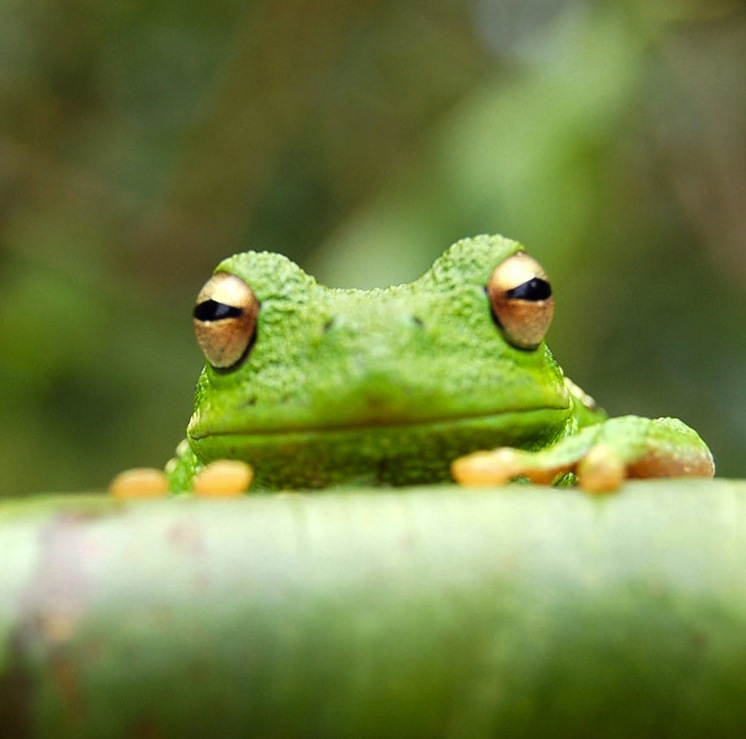
\includegraphics[width=8cm]{Images/frog.jpg}
\end{figure}


\subsection{Requirements and Specifications}

We have a setup time that includes many procedures.
So we do not have a lot of time for training and processing.
We receive our data in two different streams.
A first stream composed of 8 channels that lasts 1 minute.
A second stream with the remaining 8 channels that lasts again 1 minute.
Also our setup is composed of small micro-controllers that can perform little to no calculation.
We have to keep in mind a few things.
\begin{itemize}
\item We cannot train after having received the data cause it would take too much time
\item We cannot train beforehand a specific model since the data we have is different from the one we will receive.
\item Possibility is to train a very general auto encoder that can compress data and add some sort of de-noise by removing the wrong information.
\item and like this.
\end{itemize}

However, there is a problem in the previous studies. The effect of the same algorithm on different subjects is quite different. Research on reducing the impact of differences between individuals on the classification performance is the core work of this paper.
{DWT and CNN based multi-class motor imagery electroencephalographic signal recognition}

Because of these restrictions the best methodology is an online approach that can evaluate the channels either while we are receiving them or right after the transmission is over.
Cross-Correlation Based Discriminant Criterion emerges as the best solution [Cross-Correlation Based Discriminant Criterion for
Channel Selection in Motor Imagery BCI Systems], especially when paired with a CNN classifier such as the ENGNet we implemented based on [] as shown in this review at 1.2.[https://www.ncbi.nlm.nih.gov/pmc/articles/PMC9774545/]


\subsection{Pipeline of the work}
@zhangMotorImageryRecognition2021

\begin{itemize}
\item Read data
\item Analyze by metrics that depend only on the signal itself (variance etc...) if we can
\item ASR 
\item Cross-correlate within channels
\item CNN
\item Pack the signal and send i
\end{itemize}


\subsection{Cross-correlation and evidence}
{Wavelet Coherence Based Channel Selection for Classifying Single Trial Motor Imagery}
{Cross-Correlation Based Discriminant Criterion for
Channel Selection in Motor Imagery BCI Systems}
XCDC measures similarity between signals by
cross-correlation, and emphasizes the electrodes that:
1) signals of the same class show larger similarity, and
2) signals of different classes differ more obviously.
After ranking the channels according to XCDC, signals
from the channels with highest discriminant criterion
are chosen as the input of a convolutional neural
network (CNN) classifier, which further evaluates the
credibility of the chosen channels by classification
accuracy. The performance of XCDC is evaluated
and compared to CCS [26] and CSP-rank and is better than both (change this).
The complexity of XCDC is quadratic. Deriving
the discriminant score D of a channel involves the
computation of cross-correlation between every pair of
trials, resulting in a quadratic complexity.


\subsection{Artifact subspace reconstruction (ASR)}
Artifact subspace reconstruction (ASR) is an automatic, online-capable, component-based method that can effectively remove transient or large-amplitude artifacts contaminating electroencephalographic (EEG) data
{Evaluation of Artifact Subspace Reconstruction for Automatic Artifact Components Removal in Multi-Channel EEG Recordings}


\subsection{Genetic Algorithm why not (BPSO) and why not in general wrapper methods}
{Filtering techniques for channel selection in motor imagery EEG applications: a survey}
{A review of channel selection algorithms for EEG signal processing}
{EEG electrode selection method based on BPSO with channel impact factor for acquisition of significant brain signal}

\subsection{Evaluation of channel selection methods by building a classifier (CNN)}

Why EEGNet...

\subsection{Overall staple}
{EEG Channel Selection Techniques in Motor Imagery Applications: A Review and New Perspectives}

\subsection{Conferene notes 5/2/24}


%-------------------------------------------------------------------------
%	BIBLIOGRAPHY
%-------------------------------------------------------------------------

\addtocontents{toc}{\vspace{2em}} % Add a gap in the Contents, for aesthetics
\bibliography{Thesis_bibliography} % The references information are stored in the file named "Thesis_bibliography.bib"

\end{document}